%!TEX program = xelatex
\documentclass[10pt]{article}
\usepackage{amsthm}
\usepackage{amssymb}
\usepackage{amsmath}
\usepackage{mathrsfs}
\usepackage{titlesec}
\usepackage{xcolor}
\usepackage{enumerate}
\usepackage{bm}
\usepackage{tikz}
\usepackage{listings}
\usetikzlibrary{arrows}
\usepackage{subfigure}
\usepackage{graphicx,booktabs,multirow}
\usepackage[a4paper]{geometry}
\usepackage{upquote}
\usepackage{float}
\usepackage{pdfpages}

\geometry{verbose,tmargin=2cm,bmargin=2cm,lmargin=2cm,rmargin=2cm}
\geometry{verbose,tmargin=2cm,bmargin=2cm,lmargin=2cm,rmargin=2cm}
\lstset{language=Matlab}
\lstset{breaklines}

\input defs.tex

\newtheorem{proposition}{Proposition}
\newtheorem{remark}{Remark}

\titleformat*{\section}{\centering\LARGE\scshape}
\renewcommand{\thesection}{\Roman{section}}
\lstset{language=Matlab,tabsize=4,frame=shadowbox,basicstyle=\footnotesize,
keywordstyle=\color{blue!90}\bfseries,breaklines=true,commentstyle=\color[RGB]{50,50,50},stringstyle=\ttfamily,numbers=left,numberstyle=\tiny,
  numberstyle={\color[RGB]{192,92,92}\tiny},backgroundcolor=\color[RGB]{245,245,244},inputpath=code}

\begin{document}

\date{\today}
\title{Introduction to Machine Learning, Fall 2023 \\
	Homework 2\\
	\small (Due Tuesday Nov. 14 at 11:59pm (CST))}
\maketitle

\begin{enumerate}[1.]


	\item \defpoints{10} [Convex Optimization Basics]
	      \begin{itemize}
		      \item[(a)] Proof any norm $f:\mathbb{R}^{n}\rightarrow\mathbb{R}$ is convex.~\defpoints{2}
		      \item[(b)] Determine the convexity (i.e., convex, concave or neither) of $f(x_1,x_2)=x_1^2/x_2$ on $\mathbb{R}\times\mathbb{R}_{>0}$.~\defpoints{2}
		      \item[(c)] Determine the convexity of $f(x_1,x_2)=x_1/x_2$ on $\mathbb{R}_{>0}^{2}$.~\defpoints{2}
			  \item[(d)] Recall Jensen's inequality $f(\mathbb{E}(X)) \leq \mathbb{E}(f(X))$ if $f$ is convex for any random variable $X$. 
			  Proof the log sum inequality: 
			  \[
				\sum_{i=1}^{n} a_i \log \frac{a_i}{b_i} \geq \left( \sum_{i=1}^{n} a_i\right) \log \frac{\sum_{i=1}^{n} a_i}{\sum_{i=1}^{n} b_i} 
			  \]
			  where $a_1,\ldots,a_n$ and $b_1,\ldots,b_n$ are positive numbers. Hints: $f(x)=x\log x$ is strictly convex.~\defpoints{4}
	      \end{itemize}


		  \textbf{Solution:}

	      \newpage

	\item \defpoints{10} [Linear Methods for Classification] 
	Consider the ``Multi-class Logistic Regression'' algorithm. Given training set 
	$\mathcal{D}=\{(x^i,y^i)\mid i=1,\ldots,n\}$ where $x^i\in \mathbb{R}^{p+1}$ is the 
	feature vector and $y^i\in \mathbb{R}^{k}$ is a one-hot binary vector indicating 
	$k$ classes. We want to find the parameter $\hat{\beta}=[\hat{\beta}_1,\ldots,\hat{\beta}_k]\in \mathbb{R}^{(p+1)\times k}$ 
	that maximize the likelihood for the training set. Introducing the softmax 
	function, we assume our model has the form 
	\[
		p(y_c^i=1\mid x^i;\beta) = \frac{\exp(\beta_c^\top x^i)}{\sum_{c'}\exp(\beta_{c'}^\top x^i)},
	\]
	where $y_c^i$ is the $c$-th element of $y^i$.
		  \begin{itemize}
			\item[(a)] Complete the derivation of the conditional log likelihood for our model, which is
			\begin{align*}
				\ell(\beta) = \ln \prod_{i=1}^{n} p(y_t^i\mid x^i;\beta)
				=\sum_{i=1}^{n}\sum_{c=1}^{k}\left[ y_c^i(\beta_c^\top x^i) - y_c^i\ln \left(\sum_{c'}\exp(\beta_{c'}^\top x^i) \right)\right].
			\end{align*}
			For simplicity, we abbreviate $p(y_t^i=1\mid x^i;\beta)$ as $p(y_t^i\mid x^i;\beta)$, where 
			$t$ is the true class for $x^i$.~\defpoints{4}
			\item[(b)] Derive the gradient of $\ell(\beta)$ w.r.t. $\beta_1$, i.e., 
			\[
				\nabla_{\beta_1}\ell(\beta) = \nabla_{\beta_1} \sum_{i=1}^{n}\sum_{c=1}^{k}\left[ y_c^i(\beta_c^\top x^i) - y_c^i\ln \left(\sum_{c'}\exp(\beta_{c'}^\top x^i) \right)\right].
			\]
			Remark: Log likelihood is always concave; thus, we can optimize our model 
			using gradient ascent. (The gradient of $\ell(\beta)$ w.r.t. $\beta_2,\ldots,\beta_k$ is similar, you don't need to write them)~\defpoints{6}
		  \end{itemize}
		  \textbf{Solution:}

	      \newpage

	\item \defpoints{10} [Probability and Estimation]
	Suppose $\mathcal{D}=\{ x_{1}, x_{2}, \ldots, x_{n} \}$ are i.i.d. samples from exponential distribution with parameter 
	$\lambda > 0$, i.e., $X \sim \text{Expo}(\lambda)$. Recall the PDF of exponential distribution is
	\[
		p(x\mid \lambda) = \begin{cases}
		\lambda e^{-\lambda x},&\quad x > 0 \\
		0,&\quad \text{otherwise}
		\end{cases}.
	\]
	      \begin{itemize}
			\item[(a)] To derive the posterior distribution of $\lambda$, we assume its prior 
			distribution follows gamma distribution with parameters $\alpha,\beta > 0$, i.e., 
			$\lambda \sim\text{Gamma}(\alpha,\beta)$ (since the range of gamma distribution 
			is also $(0,+\infty)$, thus it's a plausible assumption). The PDF of $\lambda$ is 
			given by
			\[
				p(\lambda\mid \alpha,\beta) = \frac{\beta^{\alpha}}{\Gamma(\alpha)} \lambda^{\alpha-1}e^{-\lambda\beta},
			\]
			where $\Gamma(\alpha) = \int_{0}^{+\infty} t^{\alpha-1}e^{-t}dt,\ \alpha>0$. 
			Show that the posterior distribution $p(\lambda\mid \mathcal{D})$ is also a 
			gamma distribution and identify its parameters. Hints: Feel free to drop 
			constants. \defpoints{4}

			\item[(b)] Derive the maximum a posterior (MAP) estimation for $\lambda$ 
			under $\text{Gamma}(\alpha,\beta)$ prior. \defpoints{3}
			
			\item[(c)] For exponential distribution $\text{Expo}(\lambda)$, $\sum_{i=1}^{n} x_{i}\sim \text{Gamma}(n,\lambda)$ 
			and the inverse sample mean $\frac{n}{\sum_{i=1}^{n} x_{i}}$ is the MLE for $\lambda$. 
			Argue that whether $\frac{n-1}{n}\hat{\lambda}_{MLE}$ is unbiased ($\mathbb{E}(\frac{n-1}{n}\hat{\lambda}_{MLE})=\lambda$). 
			Hints: $\Gamma(z+1)=z\Gamma(z)$, $z > 0$. \defpoints{3}
	      \end{itemize}

      	  
      	  \textbf{Solution:}
      	  
      	  \newpage

	\item \defpoints{10} [Graphical Models]
	Given the following Bayesian Network, 
	\begin{figure}[h]
		\label{fig:bn}
		\vskip 0.2in
		\begin{center}
		\centerline{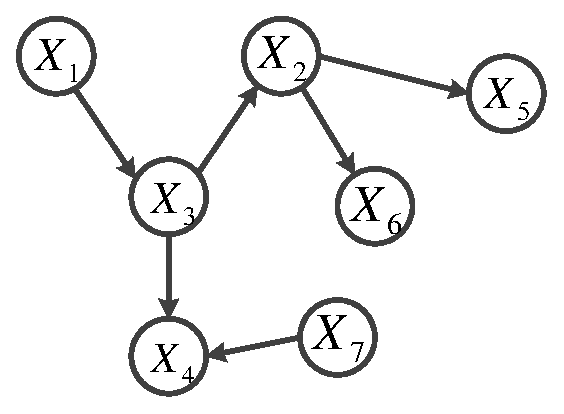
\includegraphics[width=0.4\columnwidth]{figures/bn}}
		%\caption{}
		\end{center}
		\vskip -0.2in
	\end{figure}

	answer the following questions.
		\begin{itemize}
			\item[(a)] Factorize the joint distribution of $X_{1},\cdots,X_{7}$ according 
			to the given Bayesian Network.~\defpoints{2} 
			\item[(b)] Justify whether $X_{1}\perp X_{5}\mid X_{2}$?~\defpoints{2} 
			\item[(c)] Justify whether $X_{5}\perp X_{7}\mid X_{3},X_{4}$?~\defpoints{2} 
			\item[(d)] Justify whether $X_{5}\perp X_{7}\mid X_{4}$?~\defpoints{2} 
			\item[(e)] Write down the variables that are in the Markov blanket of $X_{3}$.~\defpoints{2} 
		\end{itemize}

		\textbf{Solution:}

\end{enumerate}

\end{document}